%!TEX root = ../../../thesis.tex

\chapter{Supplement networks}

This document contains figures supplementing the main manuscript. Note that the full body of results is available online at the \href{http://smgr.mpi-inf.mpg.de}{Slime Mold Graph Repository}. 


\begin{figure}[!htbp]
\begin{center}%
  \includegraphics[width=0.75\textwidth]{path_length/physical_edge_length_histogram_cummulative_motion22.png}
\end{center}%
\caption[Goodness-of-fit plots: path lengths]{Goodness-of-fit plots of fitting the empirical path length distribution of data series $22$ with various common theoretical distributions.}
\label{fig:sup::path_lengths_goodness}
\end{figure}

\begin{figure}[!htbp]
\begin{center}%
  \includegraphics[width=0.75\textwidth]{path_width/physical_edge_width_histogram_cummulative_motion35.png}
\end{center}%
\caption[Goodness-of-fit plots: path widths]{Goodness-of-fit plots of fitting the empirical average path widths distribution of data series $35$ with various common theoretical distributions.}
\label{fig:sup::path_widths_goodness}
\end{figure}

\begin{figure}[!htbp]
\begin{center}%
  \includegraphics[width=0.75\textwidth]{face_degree/dual_node_degree_histogram_cummulative_motion35.png}
\end{center}%
\caption[Goodness-of-fit plots: face degrees]{Goodness-of-fit plots of fitting the empirical face degree distribution of data series $35$ with various common theoretical distributions.}
\label{fig:sup::face_degree_goodness}
\end{figure}

\begin{figure}[!htbp]
\begin{center}%
  \includegraphics[width=0.75\textwidth]{face_area/face_area_histogram_cummulative_motion35.png}
\end{center}%
\caption[Goodness-of-fit plots: face area]{Goodness-of-fit plots of fitting the empirical face area distribution of data series $35$ with various common theoretical distributions.}
\label{fig:sup::face_area_goodness}
\end{figure}

\begin{figure}[!htbp]
\begin{center}%
  \includegraphics[width=0.75\textwidth]{face_length/face_length_histogram_cummulative_motion35.png}
\end{center}%
\caption[Goodness-of-fit plots: face circumference]{Goodness-of-fit plots of fitting the empirical face circumference distribution of data series $35$ with various common theoretical distributions.}
\label{fig:sup::face_length_goodness}
\end{figure}

\begin{figure}[!htbp]
\begin{center}%
  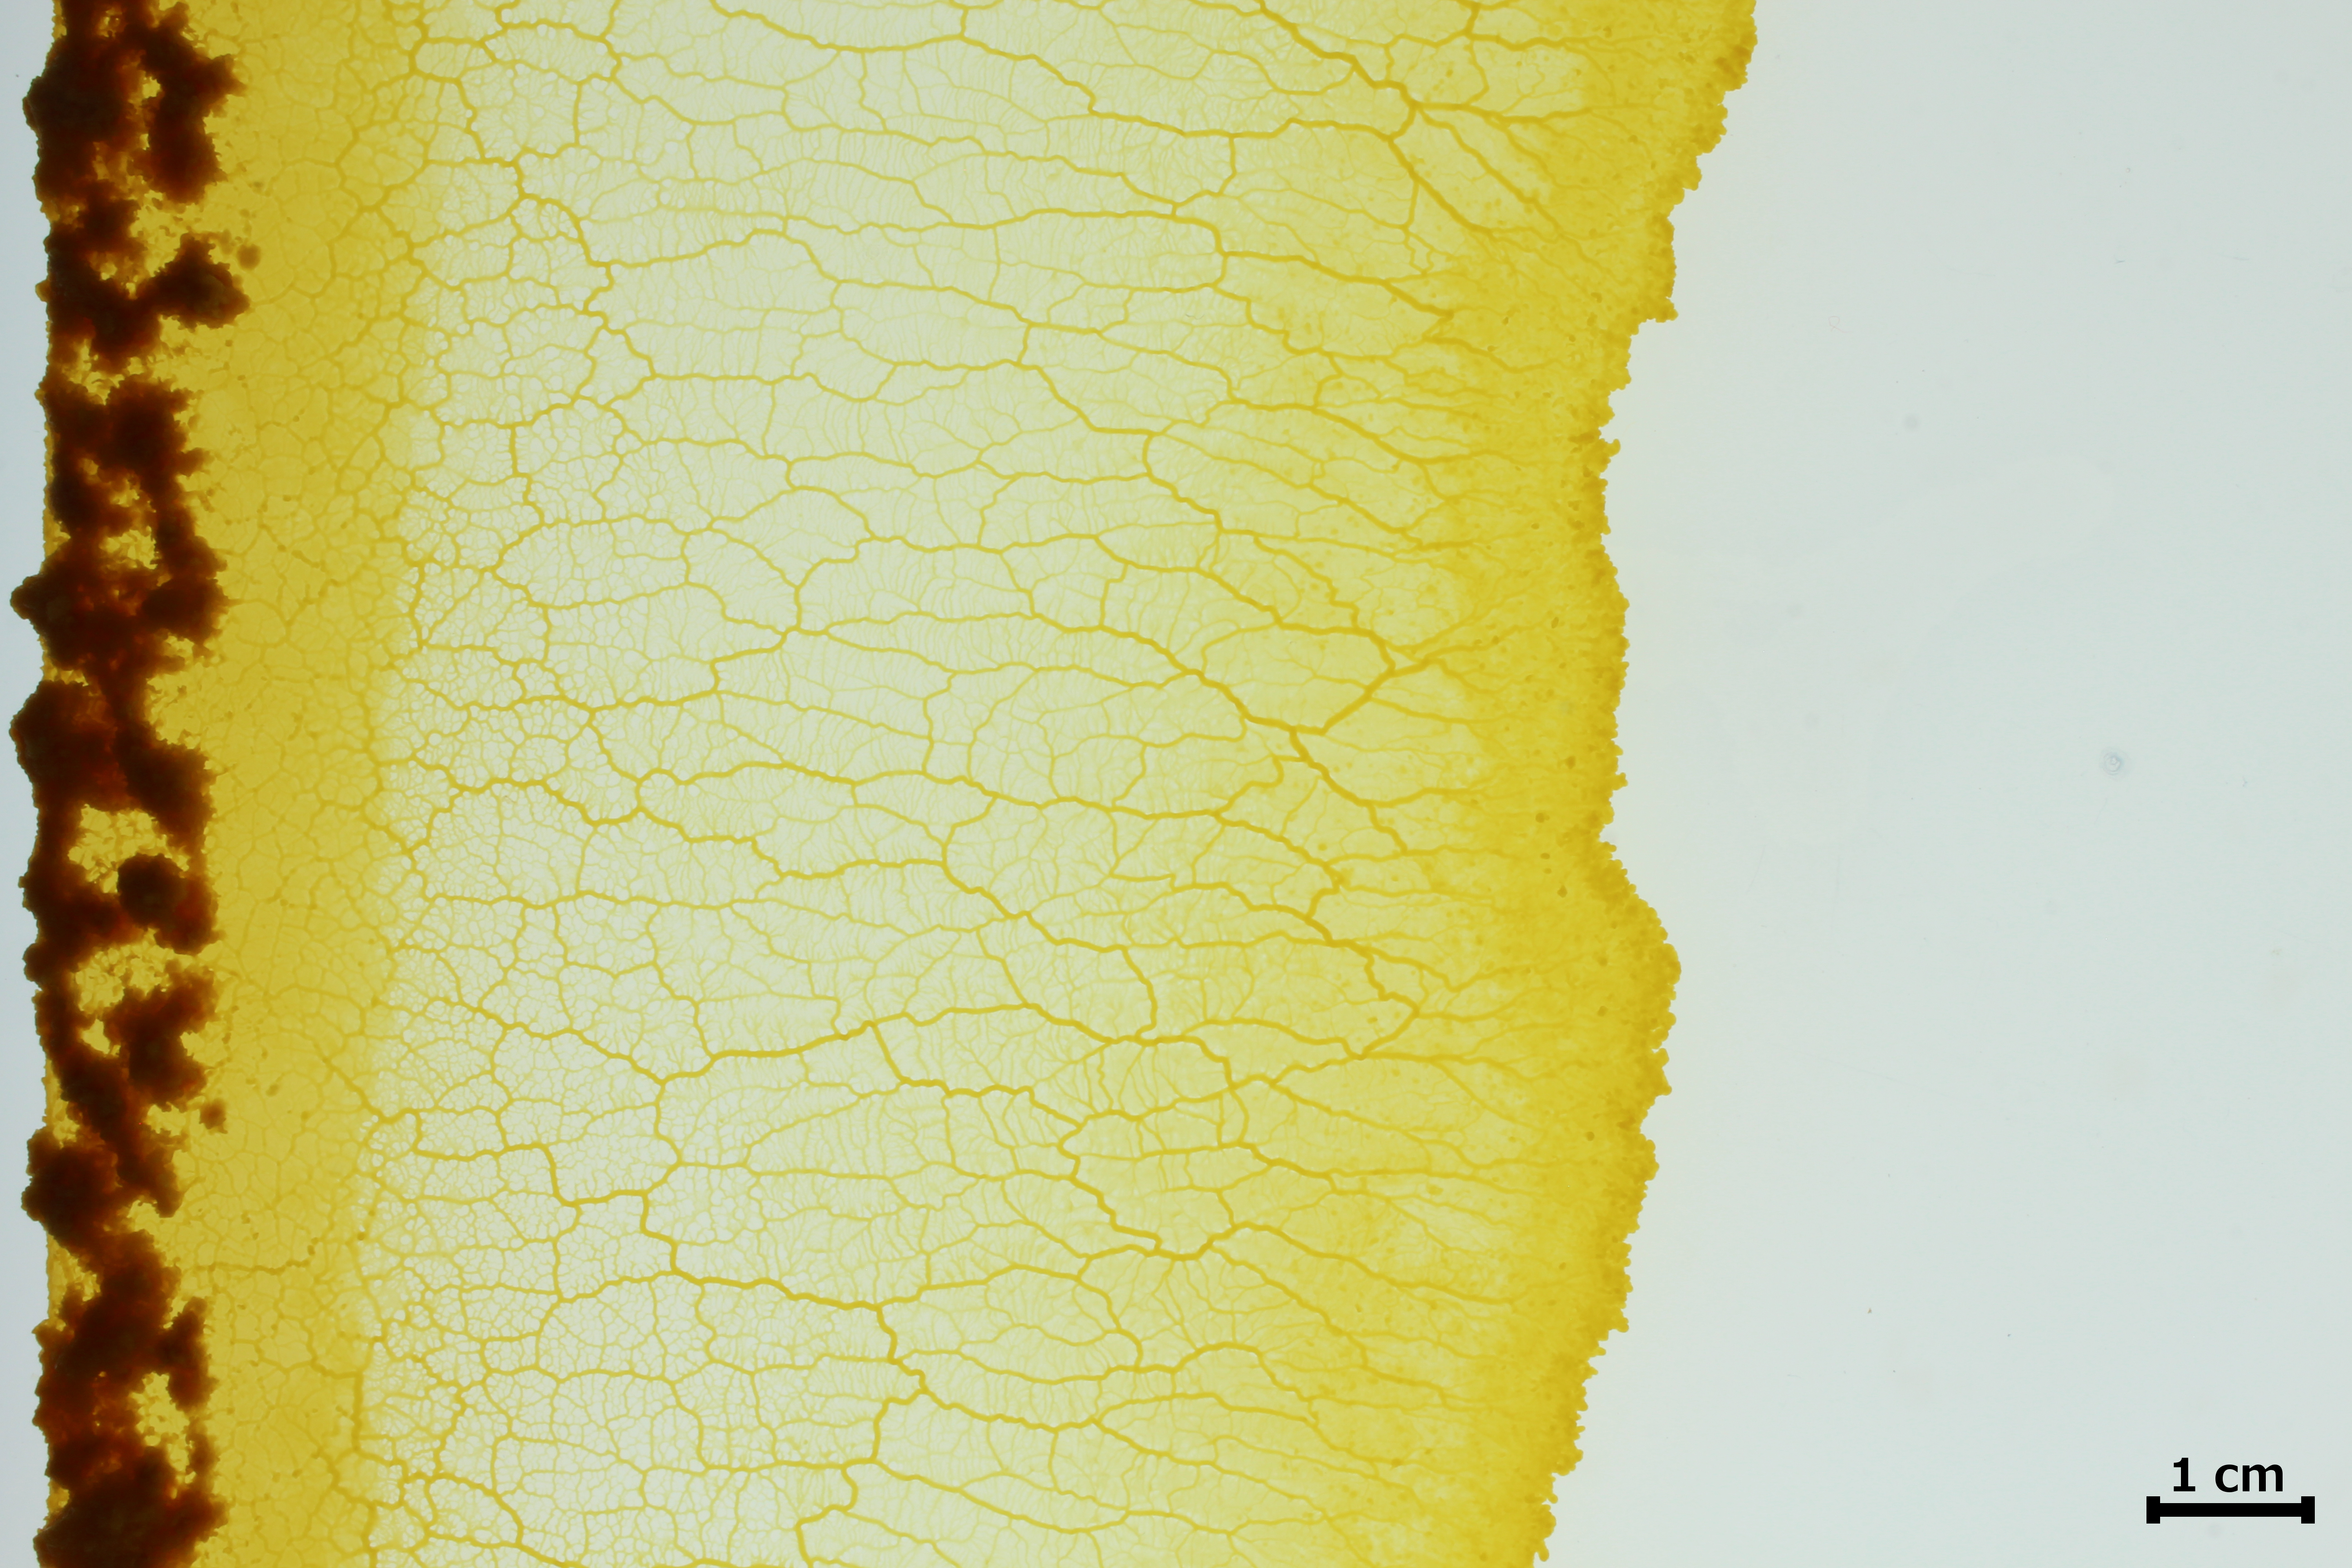
\includegraphics[width=0.75\textwidth]{cuts/physarum_sequence_2.JPG}
\end{center}%
\caption[\P advancing the apical zone]{\P advancing its growing front and expanding along the x-axis. The front itself is approximately paralell to the y-axis, i.e. perpendicular to the direction of growth. }
\label{fig:sup::physarum_expanding}
\end{figure}

\begin{figure}[!htbp]
\begin{center}%
  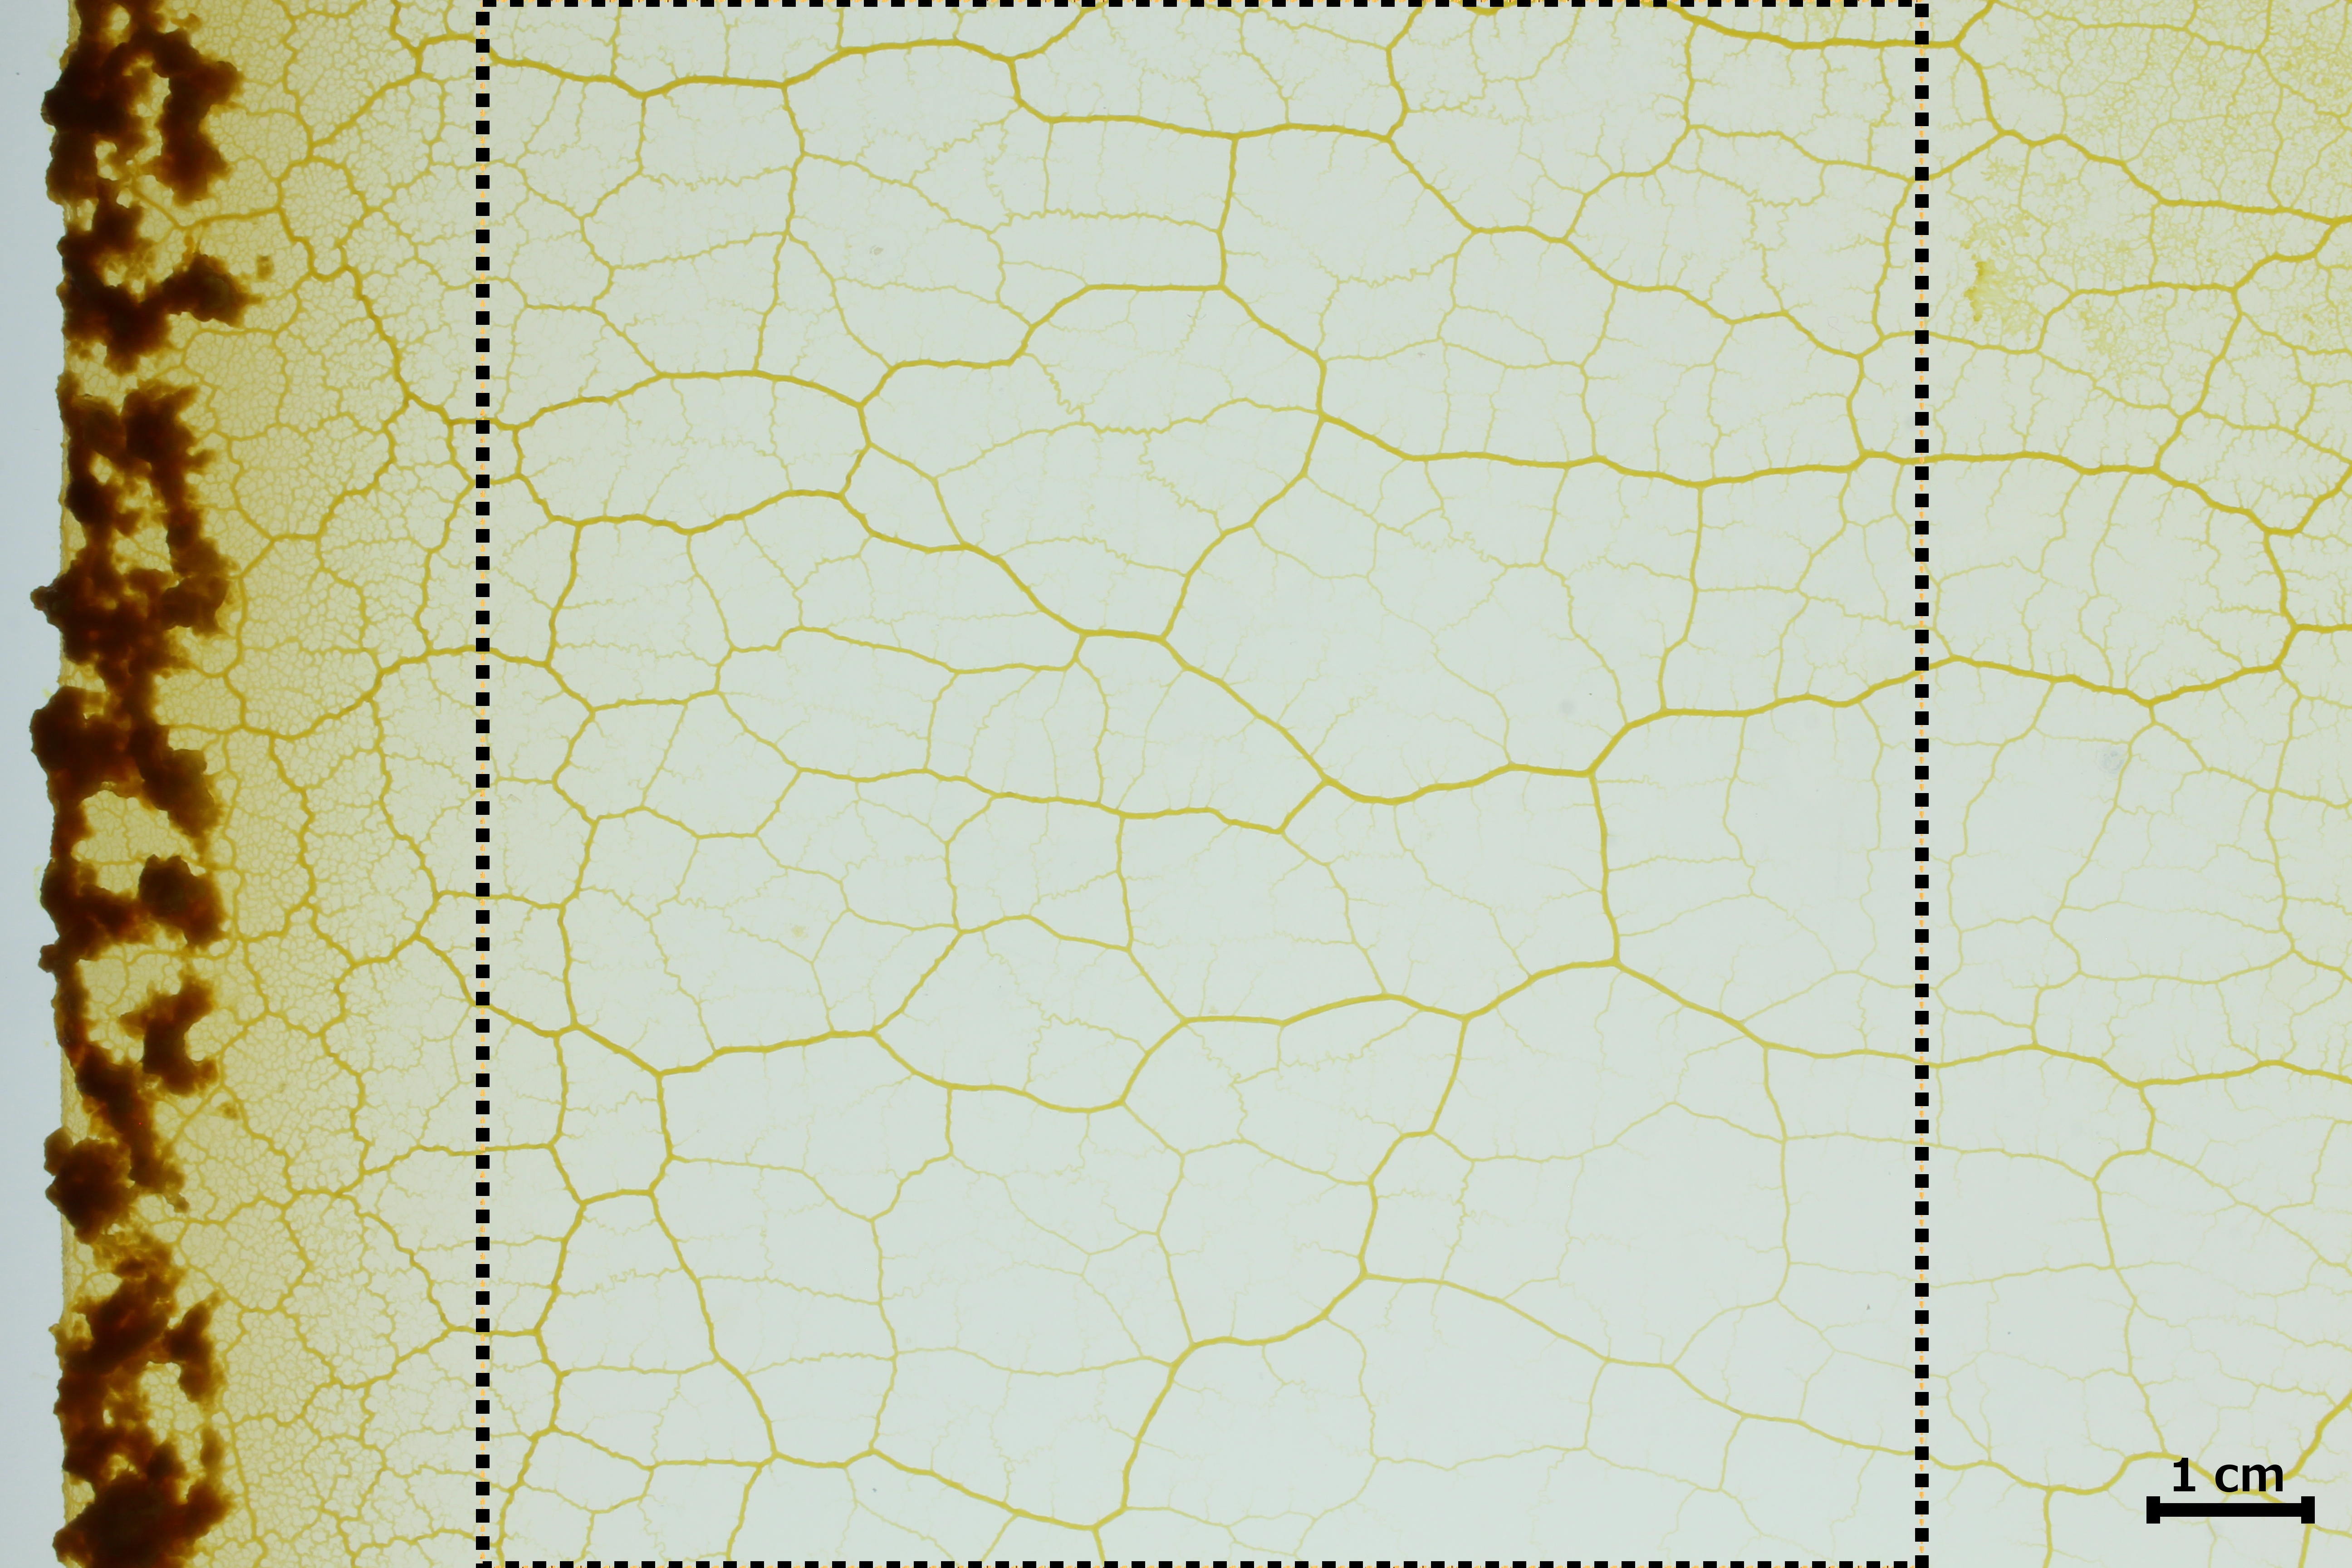
\includegraphics[width=0.75\textwidth]{cuts/physarum_sequence_4.JPG}
\end{center}%
\caption[Horizontal and vertical cuts illustrated]{After a while the growing front has escaped the area of observation leaving behing its supporting vein network. We consider the network within a predefined region of interest (dotted rectangle). We subdivide this region of interest by defining 100 equidistant vertical and horizontal lines. The intersection of the vein network with these lines define cuts. Horizontal cuts proceed from top to bottom, i.e. perpendicular to the growth direction. Vertical cuts proceed from left to right, i.e. in growth direction. Solid lines show one cut of each type.}
\label{fig:sup::physarum_roi}
\end{figure}
